\documentclass[../../main.tex]{subfiles}

\begin{document}

\section{Caracterizaci\'on de amplificadores operacionales}

En esta secci\'on se estudiar\'a c\'omo la presencia del operacional afecta a un circuito que sin \'el es puramente resistivo, lo cual permite apreciar los cambios introducidos por los polos propios de este componente. El circuito en cuesti\'on es el siguiente:\par

\begin{figure} [H]
	\centering
	\begin{circuitikz}
		
		\draw
		(5,.5) node [op amp, yscale  = -1] (opamp) {}
		(opamp.-) to [short] ($(opamp.-) + (0, -1)$)
		to [R, l_=$R_1$, *-] ($(opamp.-)+(0,-3)$) node [ground] {}
		($(opamp.+) + (-3, 0)$) node[left, *-o] {$V_{in}$}
		to [R, l_=$R_3$, *-] (opamp.+) 
		($(opamp.-) + (0, -1)$) to [R, l_=$R_2$] ($(opamp.out)+(0,-1.5)$) to [short, *-] (opamp.out)		
		to ($(opamp.out)+(1,0)$) node [right] {$V_{out}$} node[ocirc]{}
	;\end{circuitikz}

	\caption{Circuito no inversor}
\end{figure}

Los componentes utilizados fueron: \par

\begin{table} [H]
	\begin{center}
		\begin{tabular}{|l|l|l|l|}
		\hline
		Componente & Valor de la consigna	& Valor comercial ($\pm5\%$)	& Valor medido	\\
		\hline \hline
		$R_1$ 	& $2$   			& $2.2$				& $2.19$		\\ \hline
		$R_2$ 	& $160$ 			& $150$ 				& $145$		\\ \hline
		$R_3$ 	& $100$ 			& $100$				& $98$ 		\\ \hline
		\end{tabular}
	\caption{Valores de resistencias en $k\Omega$} 
	\end{center}
\end{table}

El operacional utilizado fue el \textit{LM833}, y el circuito fue armado en una \textit{protoboard}.

\subsection{An\'alisis matem\'atico con modelo de polo dominante}
Como el \'unico componente de este circuito que puede introducir polos en este circuito es el \textit{op amp} (dejando de lado capacidades e inductancias par\'asitas), la \'unica forma de obtener una respuesta en frecuencia para este circuito que no sea una constante es considerando modelos de operacionales que tomen en cuenta las singularidades de los mismos. \par

Asumiendo que entre $V^+$ y $V^-$ no circula corriente, y aplicando un divisor de tensi\'on obtenemos que:\par

 \[
	\left\{
 	\begin{array}{ll}
		V^+ = V_{in}\\
		V^- = \frac{R_1}{R_1+R_2} \cdot V_{out}
	\end{array}
	\right.
 \]

Aplicando la ecuaci\'on fundamental del operacional y simplificando, resulta que la ganancia ideal (con $A_0$ infinito) es:\par
\begin{equation} G = 1 + \frac{R_2}{R_1} = 67.21 \sim 36.5dB \end{equation}

Como el $A_0$ del operacional (seg\'un su hoja de datos) es de $110dB \sim 3.16\times 10^5 \gg G$, entonces podemos utilizar el modelo explicado en la introducci\'on para obtener la $\omega_p'$ a esta ganancia, con lo cual la funci\'on transferencia del circuito queda:

\begin{equation} \label{eq:2tf1polo} H(s) = \frac{G}{\frac{s}{\omega_p'} +1} \end{equation}

Habiendo obtenido el valor del \textit{bandwidth product} de la \textit{data sheet} del operacional, el valor de la frecuencia de corte es $f_p'= \frac{BWP}{G} \sim 238kHz$, de donde se puede completar la transferencia \ref{eq:2tf1polo} con $\omega_p'=2\pi f_p'$. El circuito tiene, entonces, un \'unico polo que se encuentra en esta frecuencia, y para $f \ll f_p'$, la ganancia deber\'ia ser igual a la ideal.\par

Por otro lado, como consideramos que no circula corriente entre las entradas inversora y no inversora del operacional, la impedancia de entrada seg\'un este modelo es infinita. \par

\subsection{M\'etodo de medici\'on}

Hasta este punto, parecer\'ia que la resistencia $R_3$ no tiene ninguna influencia en el comportamiento del circuito. Sin embargo, si consideramos que el valor de esta resistencia es de $98k\Omega$, se deber\'ia tener en cuenta que incluso una corriente del orden de los $nA$ podr\'ia provocar una ca\'ida de tensi\'on de varios $mV$. Siendo que seg\'un la hoja de datos del operacional, la corriente de \textit{bias} del circuito es t\'ipicamente de $300nA$, esperar\'iamos observar un \textit{offset} en esta resistencia de $R_3 \cdot I_{b} = 29.4mV$. Siendo que adem\'as el circuito tiene una ganancia elevada, esta peque\~na diferencia de potencial podr\'ia resultar en la salida de un \textit{offset} de aproximadamente $1.98V$, lo cual podr\'ia afectar considerablemente la saturaci\'on del circuito. \par

Para  verificar que este an\'alisis tiene m\'erito, se midi\'o la diferencia de potencial entre la entrada y la salida cuando la fase entre ellas era de $0^\circ$, que se cumpl\'ia en $f=1kHz$.

\begin{figure} [H]
	\centering
	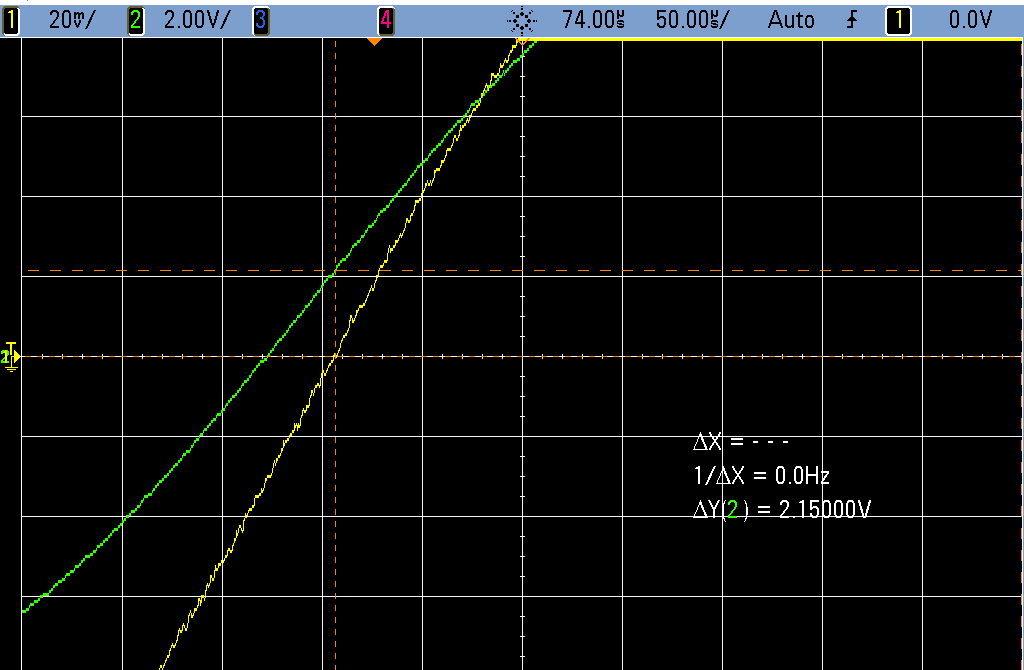
\includegraphics[scale=0.5]{fotos/tc_tp2_ej2_offset.png}
	\caption{\textit{Offset} entre la salida y la entrada cuando $\phase{H(f)|}=0^\circ$}
\end{figure}

Efectivamente, se obtuvo un \textit{offset} de 2.15V en esta medici\'on. La discrepancia entre lo calculado y lo obtenido podr\'ia provenir de una corriente de \textit{bias} superior a la t\'ipica: una corriente de $327nA$ explicar\'ia perfectamente el resultado obtenido, y la informaci\'on aportada por el fabricante indica que este valor puede llegar hasta los $750nA$, con lo cual parecer\'ia un valor razonable. A su vez, parte de la tensi\'on continua que se ve amplificada podr\'ia deberse a una $V_{DC}$ par\'asita del generador utilizado, ya que $2.5mV$ extra en la entrada tambi\'en explicar\'ian el resultado obtenido. Cualquiera de estos dos factores, o una combinaci\'on de ambos, podr\'ia estar influyendo en el resultado.\par

Debido a este fen\'omeno, se debi\'o trabajar con un \textit{offset} de alrededor de $-30mV$ a la hora de medir la respuesta en frecuencia y la impedancia de entrada del circuito (aproximadamente porque no en todas las mediciones se us\'o exactamente el mismo valor). No considerarlo llevaba a una asimetr\'ia en la saturaci\'on del operacional que limitaba la tensi\'on de entrada a\'un m\'as que lo que lo hac\'ia la gran ganancia del circuito y el \textit{slew rate}. \par


\begin{figure} [H]
	\centering
	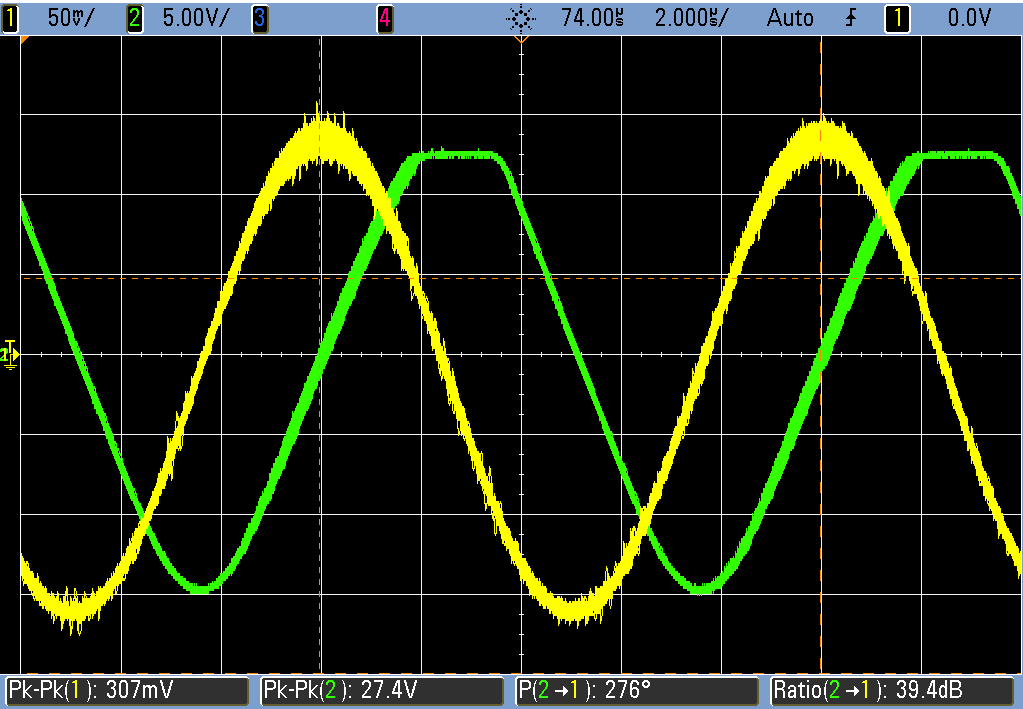
\includegraphics[scale=0.5]{fotos/tc_tp2_ej2_saturacion.png}
	\caption{Saturaci\'on producto del \textit{offset} entre la salida y la entrada}
\end{figure}

En cuanto a la impedancia de entrada, la misma se midi\'o asumiendo que la resistencia $R_3$ pod\'ia considerarse constante y con fase $0^\circ$ para todas las frecuencias, de forma tal que midiendo $V_{R_3}$, se puede obtener la corriente como $I = \frac{V_{R_3}}{R_3}$.


\subsection{An\'alisis de resultados}

\subsubsection{Respuesta en frecuencia}

Superponiendo las mediciones de respuesta en frecuencia, lo calculado con la f\'ormula \ref{eq:2tf1polo} y la simulaci\'on del circuito en \textit{LTspice}, se elaboraron los diagramas de Bode de la figura \ref{fig:hf-sin-c} \footnote{Los diagramas de bode se encuentran al final de esta secci\'on}.

Tanto el modelo utilizado para llegar a la funci\'on transferencia anal\'iticamente como el utilizado por el simulador predicen que en la frecuencia de corte debe observarse un polo de primer orden. Sin embargo, las mediciones indican la presencia de un polo de segundo orden, donde los dos polos son complejos conjugados debido al sobrepico que se presenta. \par

Efectivamente este circuito est\'a presentando otro polo adem\'as del dominante del capacitor. Una explicaci\'on que se podr\'ia ofrecer yace en la capacidad entre $V^+$ y $V^-$, o \textit{differential input capacitance}, que el fabricante estima en $12pF$. Planteado con la presencia de este capacitor, las ecuaciones del circuito resultan:\par

\begin{figure} [H]
	\centering
	\begin{circuitikz}
		
		\draw
		(5,.5) node [op amp, yscale  = -1] (opamp) {}
		(opamp.-) to [short] ($(opamp.-) + (-1, 0)$)
	%	(opamp.+)  to [R, l_=$R_3$, *-] (2,2) to node [left] {V_{in}}
	%	(opamp.out) to [short, *-o]
	%	to (7,.5) node [right] {$V_{out}$}
		($(opamp.+) + (-3, 0)$) node[left] {$V_{in}$} 
		to [R, l_=$R_3$, i = $I_3$, *-] ($(opamp.+) +(-1,0)$)
		to [C=$C$, *-]($(opamp.-)+(-1,0)$)
		to [short, *-](opamp.-)
		($(opamp.+) +(-1,0)$) to [short, *-](opamp.+)	
		($(opamp.-) + (-1, 0)$) to [short, *-] ($(opamp.-) + (-1, -1)$) 
		to [R, l_=$R_1$, *-, i=$I_1$] ($(opamp.-)+(-1,-3)$) node [ground] {}
		($(opamp.-) + (-1, -1)$) to [R, l_=$R_2$, i_<=$I_2$] ($(opamp.out)+(0,-1.5)$) to [short] (opamp.out)		
		to ($(opamp.out)+(1,0)$) node [right, -*] {$V_{out}$}
	;\end{circuitikz}

	\caption{Circuito considerando la \textit{differential input capacitance}}
\end{figure}


 \[
	\left\{
 	\begin{array}{ll}
		V_{in} = V^+ + I_3 \cdot R_3 \\
		V^+ = V^- + I_3 \cdot \frac{1}{sC} \\
		V_{out} = I_2 \cdot R_2 + V^- \\
		V_{out} = A_{vol}(s) \cdot (V^+ - V^-) \\
		V^- = I_1 \cdot R_1 \\
		I_1 = I_2 + I_3
	\end{array}
	\right.
 \]

Resolviendo el sistema, la nueva funci\'on transferencia se obtiene como:\par

\begin{equation} \label{eq:tf-con-c}
	H(s) = \left( \frac{A_0 \cdot (R_1+R_2)}{R_2+A_0\cdot (R_1+1)} \right) \cdot \left( \frac{1} {  \frac{K}{\omega_p \cdot (R_2+A_0\cdot (R_1+1))} \cdot s^2 + \frac{ (\omega_p\cdot K + R_1+R_2) }{\omega_p \cdot (R_2+A_0\cdot( R_1+1)}\cdot s + 1 } \right) 
\end{equation}

En la expresi\'on anterior, llamamos $K = C\cdot ( R_1\cdot R_2 + R_3 (R_1 +R_2 ))$. Notamos que el t\'ermino constante es id\'entico al que hab\'iamos obtenido sin considerar el capacitor, que aproximadamente la ganancia ideal del circuito. \par

Simulando con $C=12pF$, se obtienen los resultados de la figura \ref{fig:hf-con-c}.\par

El modelo predice la presencia de un sobrepico, pero sin embargo no se llega a ajustar exactamente a lo que se midi\'o. Esto puede deberse a que para un valor tan bajo de $C$, cualquier capacidad par\'asita presente en el circuito puede influir en el resultado obtenido. Por ejemplo, si consider\'asemos que podemos tener otros $10pF$ provenientes de la \textit{protoboard}, y que la capacidad del operacional es de $14pF$ en lugar de $12pF$ (ya que el fabricante indica que son 12, pero no aporta valores m\'aximos ni con cu\'anto error ni en qu\'e condiciones fueron medidos), la capacidad podr\'ia llegar a resultar incluso el doble. \par

Estudiaremos el efecto de los errores de aproximaci\'on con un an\'alisis Montecarlo. Simulando el circuito con las puntas del osciloscopio, el capacitor de $12pF$ con tolerancia $5\%$ para todos los componentes del circuito, el resultado que se obtiene es:

\begin{figure} [H]
	\centering
	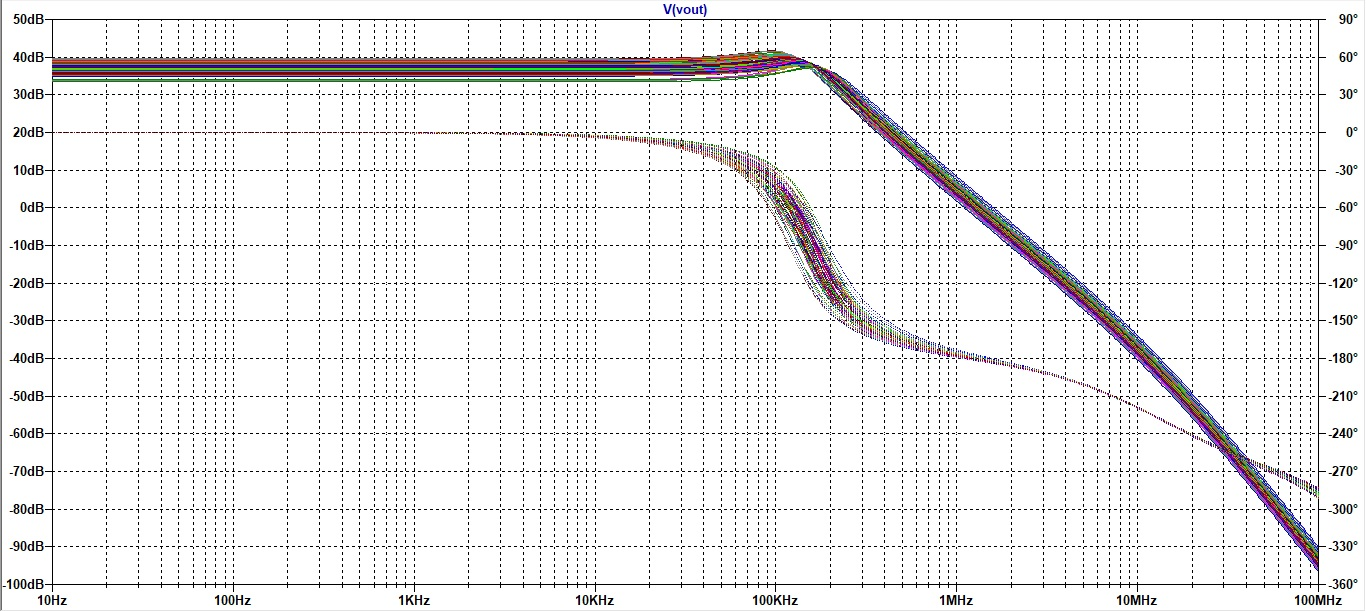
\includegraphics[scale=0.4]{fotos/tc_tp2_ej2_mc_bode.jpg}
	\caption{An\'alsis de Montecarlo de la respuesta en frecuencia}
	\label{fig:hf-con-c}
\end{figure}

Siendo que se observan picos de hasta $42dB$, concluimos que los resultados obtenidos pueden explicarse con el modelo utlilizado si tenemos en cuenta el error en el valor de los componentes.\par

Cabe destacar que en la funci\'on \ref{eq:tf-con-c}, si $R_3=50\Omega$ (del generador), la funci\'on no s\'olo no presenta un sobrepico, sino que el segundo polo no se aprecia en absoluto en este rango de frecuencias. Esto quiere decir que la presencia de una resistencia de $100k\Omega$ a la entrada, que seg\'un los modelos estudiados no deber\'ia afectar el comportamiento del circuito, ocasiona que un factor que de otra forma ser\'ia despreciable lleve la respuesta en frecuencia observable de primer orden a segundo orden.

\subsubsection{Impedancia de entrada}
Si consideramos que la impedancia entre la entrada inversora y la no inversora del operacional es infinita, entonces tambi\'en deber\'ia serlo la impedancia de entrada del circuito. Sin embargo, al estar midiendo una impedancia tan grande, debemos considerar que ya comienza a afectar las mediciones considerablemente la presencia de las puntas del osciloscopio. Como se utizaron en configuraci\'on $x10$, conectarlas al circuito implica poner en paralelo un capacitor de $C_{osc}\sim10pF$ y una resistencia de $R_{osc}\sim10M\Omega$. A su vez, con impedancias de este orden tampoco es razonable considerar que no entra ninguna corriente por el operacional. Deben tenerse en cuenta tambi\'en, pues, los $C=12pF$ que informa el fabricante que hay entre $V^+$ y $V^-$, que quedar\'an en serie con $R_1$ .

La impedancia de entrada que utilizaremos es entonces:

\begin{equation} \label{eq:ej2-zin}
	Z_{in}(s) = \frac{ C_{osc} C R_{osc} R_1 R_3 \cdot s^2 + [ R_3 \cdot (C_{osc} R_{osc} + C R_1 + C R_{osc})  + R_{osc} C R_1] \cdot s + R_3 + R_{osc} }
						{ C_{osc} C R_{osc} R_1 \cdot s^2 + (C_{osc} R_{osc} + C R_1 + C R_{osc}) \cdot s + 1}
\end{equation}

Con esta funci\'on, simulando en \textit{Spice} con las tres puntas utilizadas (antes $R_3$, despu\'es de $R_3$ y en la salida para controlar que no se sature), se obtiene el diagrama de bode de la figura \ref{fig:ej2-zin}

El modelo utilizado por el simulador se asemeja m\'as a los resultados obtenidos que el que respresenta la ecuaci\'on \ref{eq:ej2-zin}, sobre todo en la fase. Esto podr\'ia indicar que en \textit{Spice} se est\'an teniendo en cuenta par\'ametros adicionales del operacional, como por ejemplo el segundo polo de $A_{vol}(s)$, que sabemos que existe porque la \textit{unity gain frequency} ($9MHz$) no es igual al \textit{bandwidth product} ($16MHz$). Sin embargo, la forma de la funci\'on medida se respeta en ambos casos.\par

\subsection{Conclusiones}

Si bien los modelos de operacional discutidos en la introducci\'on resultan \'utiles en muchos casos, es importante tener presente qu\'e suposiciones se est\'an haciendo cuando se los utiliza y si las mismas son v\'alidas en cada circuito que se utiliza en particular. En este caso, la presencia de una resistencia de $100k\Omega$ a la entrada provoc\'o que no se pudiese despreciar el efecto de la corriente de \textit{bias}, que produc\'ia un \textit{offset} de $2V$ a la salida, as\'i como que el efecto de la capacidad par\'asita del operacional fuera apreciable, resultando que el circuito presentara dos polos complejos conjugados en lugar de primer orden. No conocer la existencia de un sobrepico en un circuito podr\'ia ocasionar garrafales errores en ganancia en la frecuencia de corte y \textit{overshoot} en el transitorio, con lo cual es importante tener en cuenta estos par\'ametros a la hora de dise\~nar circuitos.\par

\begin{figure} [H]
	\centering
	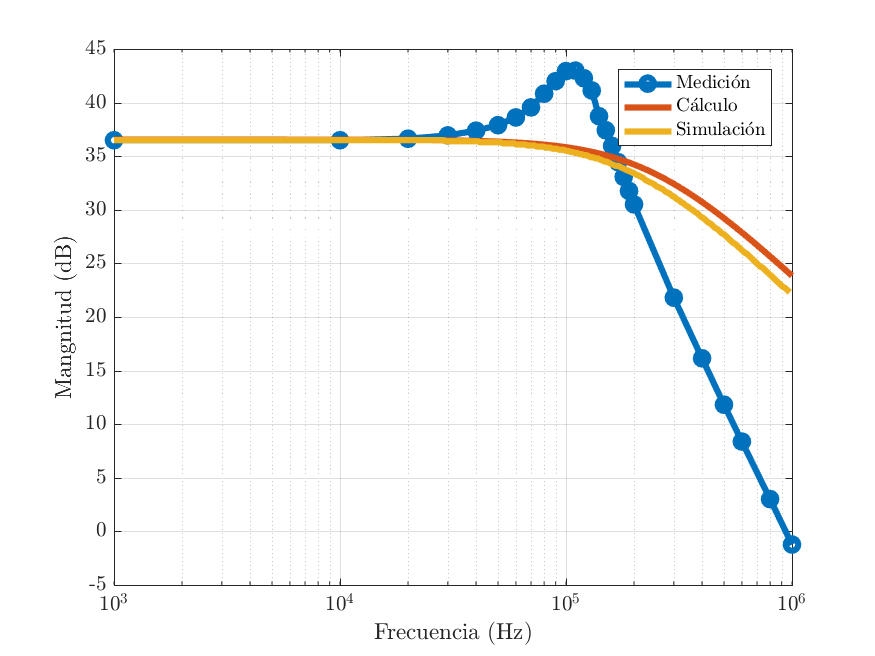
\includegraphics[scale=0.8]{fotos/tc-tp2-ej2-bode-sin-c-mag.png}
	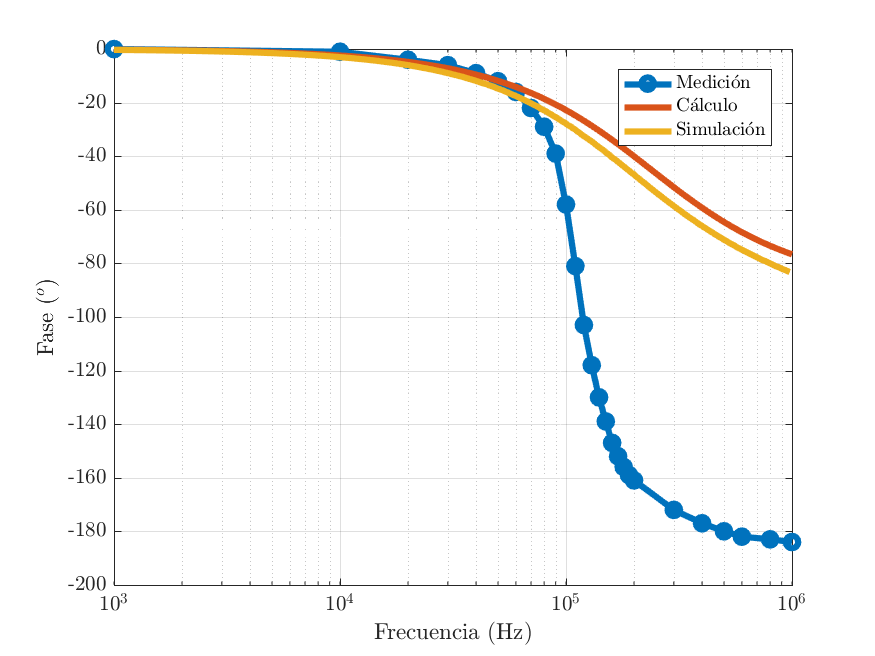
\includegraphics[scale=0.8]{fotos/tc-tp2-ej2-bode-sin-c-fase.png}
	\caption{Respuesta en frecuencia seg\'un modelo $A_{vol}(s)$}
	\label{fig:hf-sin-c}
\end{figure}

\begin{figure} [H]
	\centering
	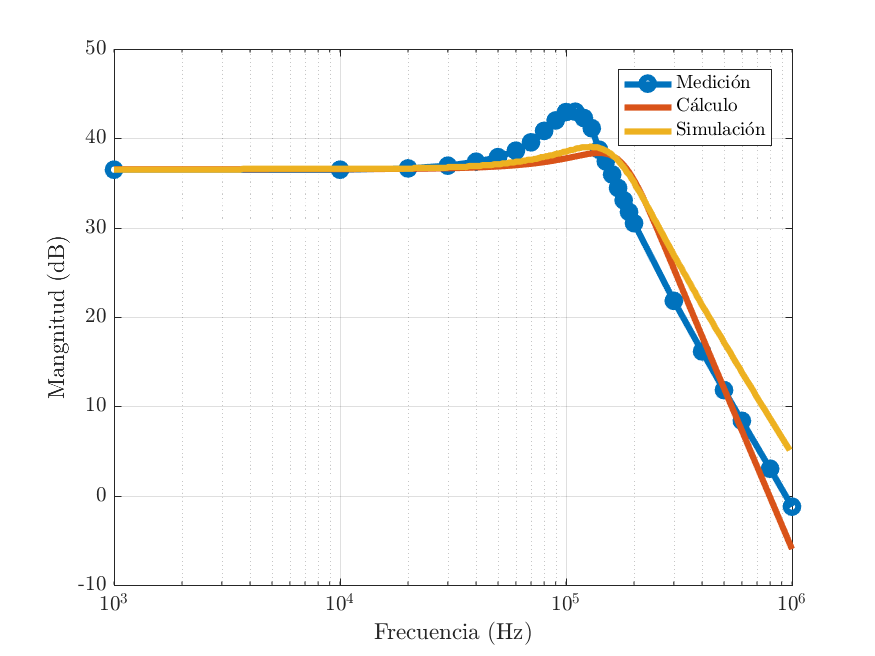
\includegraphics[scale=0.75]{fotos/tc_tp2_ej2_bode_mag.png}
	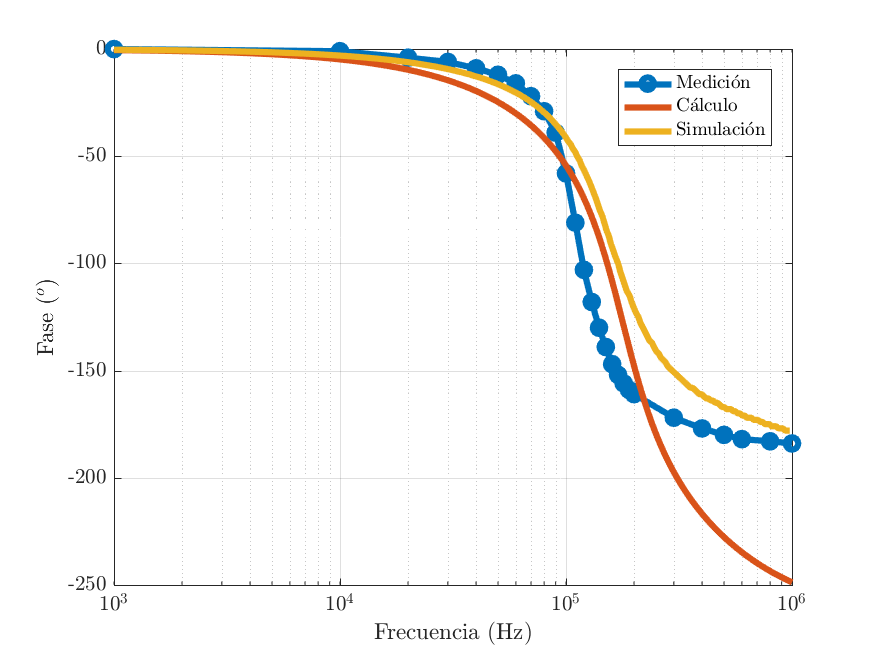
\includegraphics[scale=0.75]{fotos/tc_tp2_ej2_bode_fase.png}
	\caption{Respuesta en frecuencia considerando la \textit{differential input capacitance}}
	\label{fig:hf-con-c}
\end{figure}

\begin{figure} [H]
	\centering
	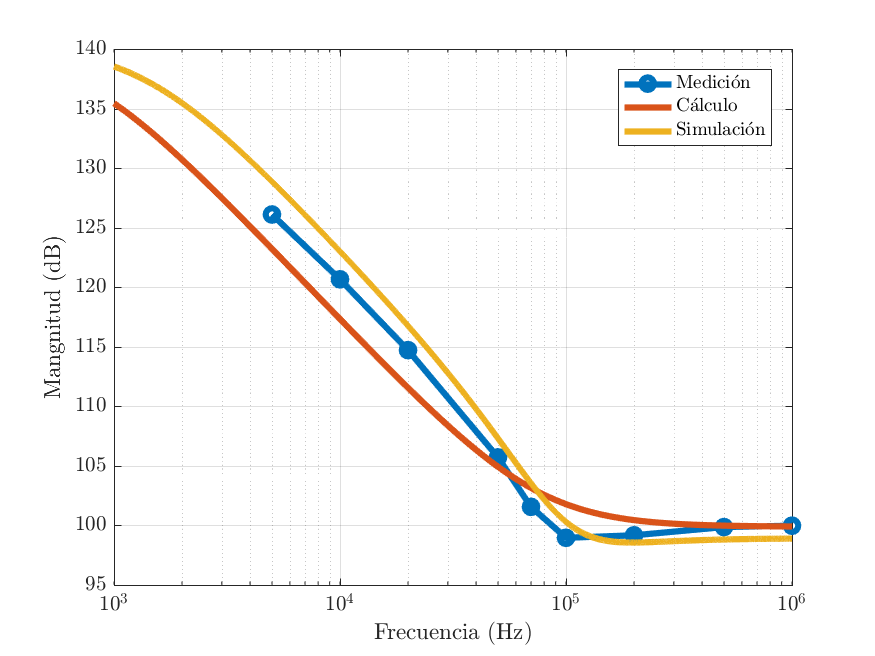
\includegraphics[scale=0.75]{fotos/tc_tp2_ej2_Zin_mag.png}
	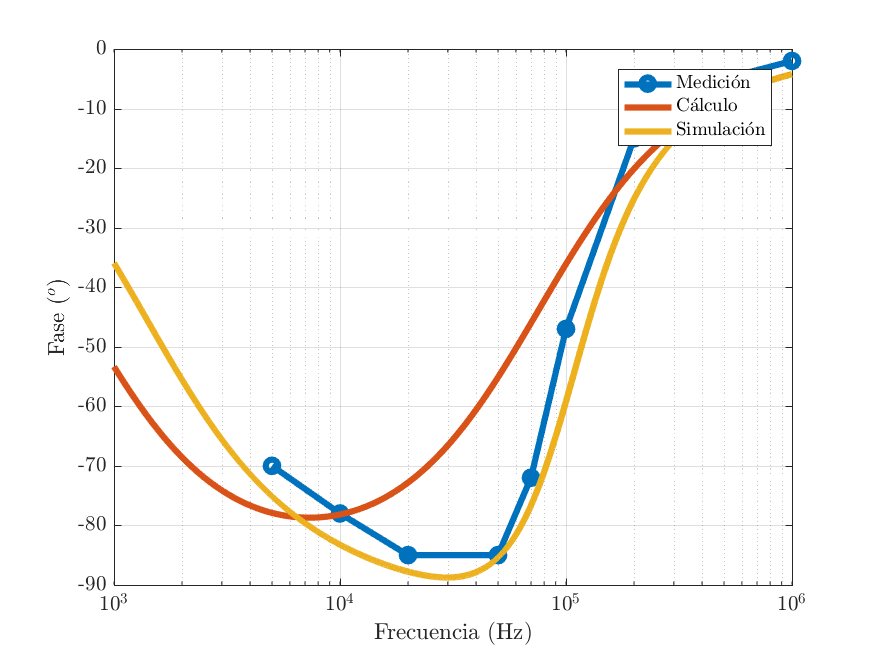
\includegraphics[scale=0.75]{fotos/tc_tp2_ej2_Zin_fase.png}
	\caption{Impedancia de entrada}
	\label{fig:ej2-zin}
\end{figure}

\end{document}

